\documentclass[12pt]{article}
\usepackage[utf8]{inputenc}
\usepackage[T1]{fontenc}
\usepackage{amsmath}
\usepackage{amsfonts}
\usepackage{amssymb}
\usepackage[version=4]{mhchem}
\usepackage{stmaryrd}
\usepackage{physics}

\usepackage{listings} % Required for insertion of code
\usepackage{xcolor} % Required for custom colors

% Define custom colors
\definecolor{codegreen}{rgb}{0,0.6,0}
\definecolor{codegray}{rgb}{0.5,0.5,0.5}
\definecolor{codepurple}{rgb}{0.58,0,0.82}
\definecolor{backcolour}{rgb}{0.95,0.95,0.92}

% Setup the style for code listings
\lstdefinestyle{mystyle}{
    backgroundcolor=\color{backcolour},   
    commentstyle=\color{codegreen},
    keywordstyle=\color{magenta},
    numberstyle=\tiny\color{codegray},
    stringstyle=\color{codepurple},
    basicstyle=\ttfamily\footnotesize,
    breakatwhitespace=false,         
    breaklines=true,                 
    captionpos=b,                    
    keepspaces=true,                 
    numbers=left,                    
    numbersep=5pt,                  
    showspaces=false,                
    showstringspaces=false,
    showtabs=false,                  
    tabsize=2
}

% Activate the style
\lstset{style=mystyle}
\usepackage{graphicx}


\title{Ch/ChE 164 Winter 2024 \\
 Homework Problem Set \#7 \\
 Due Date: Thursday, March 7, 2024 @ 11:59pm PT \\
 Out of 100 Points \\
 Project - Work on Questions 1 and 2 }

\author{}
\date{}


\begin{document}
\maketitle
\section{}
\begin{enumerate}
  \item The Gibbs-Bogoliubov-Feynmann (GBF) variational principle can be used to approximately evaluate integrals. Consider the following integral, which does not admit of an analytical closed form expression:
\end{enumerate}


\begin{equation*}
I=\int_{-\infty}^{\infty} d x \exp \left(-\frac{1}{2} a x^{2}-\frac{1}{4 !} u x^{4}\right) \tag{1}
\end{equation*}


where $a$ and $u$ are positive constants. We can regard the exponent as a "Hamiltonian"


\begin{equation*}
H=\frac{1}{2} a x^{2}+\frac{1}{4 !} u x^{4} \tag{2}
\end{equation*}


Use the GBF variational method to evaluate the integral approximately by making a reference "Hamiltonian"


\begin{equation*}
H_{R}=\frac{1}{2} A x^{2} \tag{3}
\end{equation*}

\subsection\\
(i) (10 points) Derive an expression for $A$ in terms of the parameters $a$ and $u$;\\
To start with, we can consider the inequality $I = I_R \langle \exp[-(H-H_R)] \rangle_R \geq I_R \exp[-\langle H \rangle_R + \langle H_R \rangle_R]$. We can use the reference Hamiltonian to compute the reference partition function, which is given by:
\begin{equation}
I_R=\int_{-\infty}^{\infty} \exp \left(-\frac{1}{2} A x^2\right) d x=\sqrt{\frac{2 \pi}{A}}
\end{equation}
We cognize this also as a reference partition function.
Now come we want to compute the quantities $\langle H \rangle_R$ and $\langle H_R \rangle_R$.
We can substitute our expression for $I_R$ into the expression for $\left\langle H\right\rangle_R$ to get:
\begin{equation}
\left\langle H\right\rangle_R=\sqrt{\frac{A}{2 \pi}} \int_{-\infty}^{\infty} \exp \left(-\frac{1}{2} A x^2\right) \left(\frac{1}{2} a x^2+\frac{1}{4 !} u x^4\right) d x
\end{equation}
We can make the integrand into 2 integrals by distribution:
\begin{equation}
\left\langle H\right\rangle_R=\sqrt{\frac{A}{2 \pi}} \left(\int_{-\infty}^{\infty} \exp \left(-\frac{1}{2} A x^2\right)\left(\frac{1}{2} a x^2\right) d x+\int_{-\infty}^{\infty} \exp \left(-\frac{1}{2} A x^2\right)\left(\frac{1}{4 !} u x^4\right) d x\right) = \frac{a}{2A}+ \frac{u}{8A^{2}}
\end{equation}
Next, we want to find $\left\langle H_R\right\rangle_R$, and it is given by:
\begin{equation}
\left\langle H_R\right\rangle_R=\sqrt{\frac{A}{2 \pi}} \int_{-\infty}^{\infty} \exp \left(-\frac{1}{2} A x^2\right) \left(\frac{1}{2} A x^2\right) d x = \frac{1}{2}
\end{equation}
And then we want to find the value of $A$ that maximizes the quantity $I_R \exp[-\langle H \rangle_R + \langle H_R \rangle_R]$. 
\begin{equation}
  \frac{\partial }{\partial A} \left( I_R \exp[-\langle H \rangle_R + \langle H_R \rangle_R] \right) 
\end{equation}
Minimizing this expression is equivalent to maximizing is logarithm:
\begin{equation}
  \frac{\partial }{\partial A} \left( \ln I_R - \langle H \rangle_R + \langle H_R \rangle_R \right) = 0
\end{equation}
This gives us:
\begin{equation}
  2A^{2}- 2aA - u = 0
\end{equation}
We can solve for $A$ to get:
\begin{equation}
  A = \frac{a \pm \sqrt{a^2 + 2u}}{2}
\end{equation}
from which we only keep the positive root:
\begin{equation}
  A = \frac{a + \sqrt{a^2 + 2u}}{2}
\end{equation}

\subsection\\
(ii) (5 points) Obtain an approximate expression for the integral $I$;\\\\
The maximum value for this expression is going to be bounded by:
\begin{equation}
  I \leq I_R \exp[-\langle H \rangle_R + \langle H_R \rangle_R] = \sqrt{\frac{2 \pi}{A}} \exp\left[-\frac{a}{2A} - \frac{u}{8A^{2}} + \frac{1}{2}\right]
\end{equation}
with all of these quantities as defined above.
\subsection\\
(iii) (5 points) Make a plot of the approximate expression and compare it with the numerical value of the integral for some parameter selections.
\begin{figure}
  \centering
  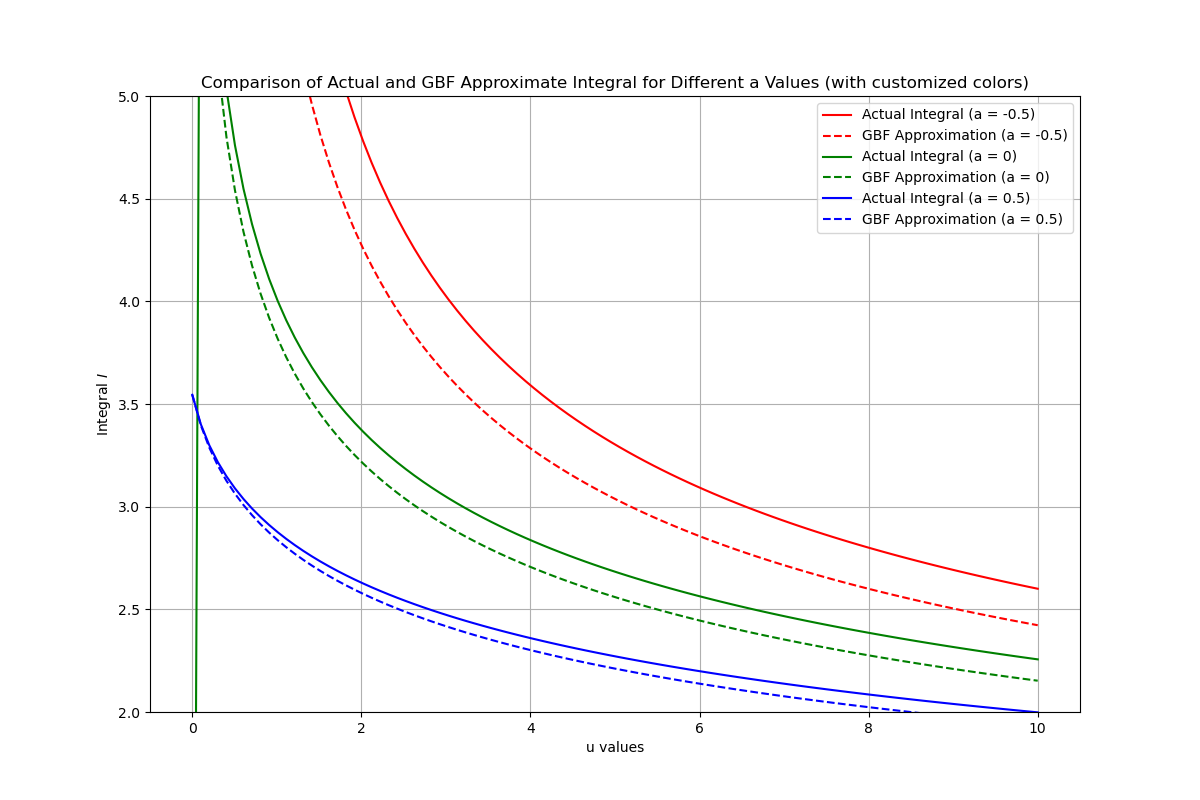
\includegraphics[width=\textwidth]{gbf_approximation.png}
  \caption{Comparison of Actual and GBF Approximate Integral for Different a Values (with customized colors)}
  \label{fig:gbf_approximation}
\end{figure}
% Inline Python code in the document
\begin{lstlisting}[language=Python]
import numpy as np
import matplotlib.pyplot as plt
from scipy.integrate import quad, IntegrationWarning

# Define the range for u
u_range = np.linspace(0.0, 10, 100)

# Parameters a for each condition
a_values = [-0.5, 0, 0.5]

# Define the actual integrand with safe checks
def exact(x, a, u):
    return np.exp(-0.5 * a * x**2 - (u/24) * x**4)

# Define the GBF approximate integral
def approximant(a, u):
    A = (a + np.sqrt(a**2 + 2*u)) / 2
    approx = np.sqrt(2 * np.pi / A) * np.exp(-a / (2*A) - u / (8*A**2) + 1/2)
    return approx

# Containers for numerical and GBF approximate results, with checks for safe computation
exact_results = {a_val: [] for a_val in a_values}
approx_results = {a_val: [] for a_val in a_values}

# Calculate the numerical and GBF approximate integrals for each a and range of u
for a_val in a_values:
    for u_val in u_range:
        # Numerical integration with error handling
        result, _ = quad(exact, -np.inf, np.inf, args=(a_val, u_val), limit=100)
        exact_results[a_val].append(result)

        # GBF approximate integral with error handling
        gbf_approx_val = approximant(a_val, u_val)
        approx_results[a_val].append(gbf_approx_val)

# Plot the results with error handling and customized colors
plt.figure(figsize=(12, 8))

# Define custom colors for clarity
colors = ['red', 'green', 'blue']

for idx, a_val in enumerate(a_values):
    actual_color = colors[idx]  # Color for the actual integral
    gbf_color = colors[idx] + '--'  # Dashed line color for GBF approximation

    plt.plot(u_range, exact_results[a_val], label=f'Actual Integral (a = {a_val})', color=actual_color, linestyle='-', marker='')
    plt.plot(u_range, approx_results[a_val], label=f'GBF Approximation (a = {a_val})', color=actual_color, linestyle='--', marker='')

# make a limit on the vertical axis
plt.ylim(2, 5)
plt.xlabel('u values')
plt.ylabel('Integral $I$')
plt.title('Comparison of Actual and GBF Approximate Integral for Different a Values (with customized colors)')
plt.legend()
plt.grid(True)
plt.savefig('gbf_approximation.png')

\end{lstlisting}
\subsection\\
(iv) (5 points) Based on your results from (iii) and (iv), comment on the effects of $a$ and $u$ on the accuracy of the GBF method.\\\\
As can be seen from the plot, thhe approximate integral is less accurate for more negative values of $a$ on a range of $u$ values.
\section{}
\begin{enumerate}
  \setcounter{enumi}{1}
  \item Simple liquid crystals are systems consisting of anisotropic, e.g., rod-like molecules. At high temperatures, the orientations of these molecules are random; this is called the isotropic phase. At low temperatures, molecules align parallel to each other; this is called the nematic phase. The simplest lattice model for this transition is a 3-state model in which a molecule can take any one of the three $(x, y, z)$ orthogonal orientations. If two nearest neighbor molecules lie parallel to each other, there is an energy gain of $-\varepsilon<0$. Otherwise there is no gain. Assuming single occupancy on each site and no vacancy, we may define variables $\sigma_{x}(i), \sigma_{y}(i), \sigma_{z}(i)$, such that $\sigma_{x}(i)=1$ if molecule $i$ lies parallel to the $x$-axis and $\sigma_{x}(i)=0$ if not, and likewise for other directions. (Of course, $\sigma_{x}(i)+\sigma_{y}(i)+\sigma_{z}(i)=1$.)
\end{enumerate}

The average $\left\langle\sigma_{\alpha}(i)\right\rangle(\alpha=x, y, z)$ gives the fraction of molecules oriented along the $\alpha$-axis. If we take the $z$-axis as the orientation in the nematic state, we may define an order parameter as


\begin{equation*}
S=\frac{1}{2}\left(3\left\langle\sigma_{z}\right\rangle-1\right) \tag{4}
\end{equation*}


such that in the isotropic state $S=0$ and in the nematic state $S>0$.

\subsection\\(i) (15 points) Construct a mean field free energy (per molecule) in terms of the order parameter $S$.\\
We can use the definition for the free energy:
\begin{equation}
F = E - TS
\end{equation}
The energy for a given molecule is given by:
\begin{equation}
E = -\varepsilon \sum_{i,j} \vec{\sigma}_i \cdot \vec{\sigma}_j 
\end{equation}
where the sum is over nearest neighbors.
Now, we only care about the average value of this product, which is given by the expansion:
\begin{equation}
\sigma^{2} \equiv \vec{\sigma}_i \cdot \vec{\sigma}_j = \langle \sigma_x \rangle^2 + \langle \sigma_y \rangle^2 + \langle \sigma_z \rangle^2
\end{equation}
We know that the value of $\langle \sigma _{z } \rangle$ is given by:
\begin{equation}
\langle \sigma_z \rangle = \frac{1}{3} (1 + 2S)
\end{equation}
We can use this to find the value of $\langle \sigma_x \rangle$ and $\langle \sigma_y \rangle$ with the constraint that $\langle \sigma_x \rangle + \langle \sigma_y \rangle + \langle \sigma_z \rangle = 1$:
\begin{equation}
\langle \sigma_x \rangle = \frac{1}{3} (1 - S)
\end{equation}
So, the $\sigma ^{2}$ term is given by:
\begin{equation}
\sigma^{2} = \frac{1}{9} (1 - S)^2 + \frac{1}{9} (1 - S)^2 + \frac{1}{9} (1 + 2S)^2 = \frac{1}{3} (1 + 2S^2)
\end{equation}
We plug this value into the above summation for the energy, multiply by a factor of $N$ since there are $N$ molecules, also motive by a factor of the coordination number $z$, and divide by 2 to take into account over counting. We get:
\begin{equation}
E = -\frac{Nz\varepsilon}{6} (1 + 2S^2)
\end{equation}
Next, we want to find the entropy. It is given by:
\begin{equation}
S = -k_B \sum_{i}^{N} \left(\langle \sigma_x \rangle \ln \langle \sigma_x \rangle + \langle \sigma_y \rangle \ln \langle \sigma_y \rangle + \langle \sigma_z \rangle \ln \langle \sigma_z \rangle\right)
\end{equation}
We can use the values of $\langle \sigma_x \rangle$, $\langle \sigma_y \rangle$, and $\langle \sigma_z \rangle$ to find the value of the entropy. We get:
\begin{equation}
S = -k_B N \left(\frac{1 - S}{3} \ln \frac{1 - S}{3} + \frac{1 - S}{3} \ln \frac{1 - S}{3} + \frac{1 + 2S}{3} \ln \frac{1 + 2S}{3}\right)
\end{equation}
Combining the 2 terms that are the same, we get:
\begin{equation}
S = -k_B N \left(\frac{2 - 2S}{3} \ln \frac{1 - S}{3} + \frac{1 + 2S}{3} \ln \frac{1 + 2S}{3}\right)
\end{equation}
So the total free energy is given by:
\begin{equation}
F = -\frac{Nz\varepsilon}{6} (1 + 2S^2) + k_B T N \left(\frac{2 - 2S}{3} \ln \frac{1 - S}{3} + \frac{1 + 2S}{3} \ln \frac{1 + 2S}{3}\right)
\end{equation}
Then, we simply have to divide by a factor of $N$ to get the free energy per molecule:
\begin{equation}
f = -\frac{z\varepsilon}{6} (1 + 2S^2) + k_B T \left(\frac{2 - 2S}{3} \ln \frac{1 - S}{3} + \frac{1 + 2S}{3} \ln \frac{1 + 2S}{3}\right)
\end{equation}
\subsection\\(ii) (10 points) Expand the free energy to 4 th order in $S$. From the form of this free energy, can you tell whether the isotropic-nematic transition is first or second order?\\\\
The main task now is to Taylor expand the natural logarithms in our free energy expression up to 4th order in $S$. 
\begin{equation}
\ln \frac{1 - S}{3} = \ln (1 - S) - \ln 3 = -\ln 3 - S - \frac{S^2}{2} - \frac{S^3}{3} - \frac{S^4}{4} - \ldots
\end{equation}
\begin{equation}
\ln \frac{1 + 2S}{3} = \ln (1 + 2S) - \ln 3 = -\ln 3 + 2S - \frac{4S^2}{2} + \frac{8S^3}{3} - \frac{16S^4}{4} + \ldots
\end{equation}
For the free energy, this gives:
\begin{equation}
f \approx \frac{S^{4} T k_{B}}{2} - \frac{S^{3} T k_{B}}{3} + S^{2} T k_{B} - \frac{S^{2} \epsilon z}{3} - T k_{B} \log{\left(3 \right)} - \frac{\epsilon z}{6} + O(S^{5})
\end{equation}
This is a first order transition, as there is no term in $S$ in the free energy expression.
% Inline Python code in the document
\begin{lstlisting}[language=Python]
from sympy import *

# Define the symbols for this expression: f = -\frac{z\varepsilon}{6} (1 + 2S^2) + k_B T \left(\frac{2 - 2S}{3} \ln \frac{1 - S}{3} + \frac{1 + 2S}{3} \ln \frac{1 + 2S}{3}\right)
f, z, S, T, epsilon, k_B = symbols('f z S T \epsilon k_B')
f = -z * epsilon / 6 * (1 + 2 * S**2) + k_B * T * ((2 - 2 * S) / 3 * log((1 - S) / 3) + (1 + 2 * S) / 3 * log((1 + 2 * S) / 3))
# use this tailor expansion for the logarithm \ln \frac{1 - S}{3} = \ln (1 - S) - \ln 3 = -\ln 3 - S - \frac{S^2}{2} - \frac{S^3}{3} - \frac{S^4}{4} - \ldots and \ln \frac{1 + 2S}{3} = \ln (1 + 2S) - \ln 3 = -\ln 3 + 2S - \frac{4S^2}{2} + \frac{8S^3}{3} - \frac{16S^4}{4} + \ldots
f = f.subs(log((1 - S) / 3), -log(3) - S - S**2 / 2 - S**3 / 3 - S**4 / 4)
f = f.subs(log((1 + 2 * S) / 3), -log(3) + 2 * S - 4 * S**2 / 2 + 8 * S**3 / 3 - 16 * S**4 / 4)
# simplify the expression
f = simplify(f)
# print the expression
print(latex(f))

\end{lstlisting}


\subsection\\(ii) (15 points) Use the approximate free energy in (ii) to find the isotropic-nematic transition temperature, the value of the order parameter for both phases at the transition, and the latent heat of the transition (the difference of energy between two states.)\\\\
For a first order transition, we know that
\begin{equation}
\frac{\partial f}{\partial S} (S^*, T^*) = \frac{\partial f}{\partial S} (0, T^*)
\end{equation}
and we know that $F(S^*, T^*) = F(0, T^*)$. We can use these two equations to solve for $T^*$ and $S^*$. Minimizing our free and energy with respect to the order perimeter gives:
\begin{equation}
- \frac{25 S^{4} T k_{B}}{2} + 2 S^{3} T k_{B} - S^{2} T k_{B} + 2 S T k_{B} - \frac{2 S \epsilon z}{3}
\end{equation}
\section{}
\begin{enumerate}
  \setcounter{enumi}{2}
  \item Consider the lattice gas model with a grand partition function
\end{enumerate}


\begin{equation*}
\Xi(\mu, V, T)=\sum_{\left\{\sigma_{i}\right\}} \exp \left\{\beta \mu \sum_{i} \sigma_{i}+\beta \varepsilon_{0} \sum_{\langle i j\rangle} \sigma_{i} \sigma_{j}\right\} \tag{5}
\end{equation*}

\subsection{}
(i) (15 points) Show that there exists a one-to-one correspondence between the parameters in the lattice gas model with those in the Ising model. In particular, show that the pressure for the lattice gas, $p$, is related to the free energy per spin of the Ising model, $f$, via


\begin{equation*}
p=-\frac{1}{2} z J+h-f \tag{6}
\end{equation*}


(We have taken the volume of a lattice site to be 1.)\\\\
We see that the chemical potential relates to the magnetic field and $\varepsilon _{0}$ relates to the coupling constant $J$, giving a one-to-one correspondence between the Hamiltonians of the lattice gas and the Ising model.
With the icing model at a certain site we had a choice of two spins $s _{i} = \pm 1$. Whereas for the lattice gas we have a choice of two states $\sigma _{i} = 0, 1$. These can be related by considering the following transformation:
\begin{equation}
\sigma _{i} = \frac{1}{2} (1 + s _{i})
\end{equation}
We can plug this into the partition function that was given for the lattes gas model:
\begin{equation}
\Xi=\sum_{\left\{\sigma_{i}\right\}} \exp \left\{\beta \mu \sum_{i} \sigma_{i}+\beta \varepsilon_{0} \sum_{\langle i j\rangle} \sigma_{i} \sigma_{j}\right\}
\end{equation}
to get:
\begin{equation}
\Xi=\sum_{\left\{s_{i}\right\}} \exp \left\{\beta \mu \sum_{i} \frac{1}{2} (1 + s_{i})+\beta \varepsilon_{0} \sum_{\langle i j\rangle} \frac{1}{4} (1 + s_{i})(1 + s_{j})\right\}
\end{equation}
We take out the constant from inside the summation in both cases and do a distributive multiplication on the second term:
\begin{equation}
\Xi=\sum_{\left\{s_{i}\right\}} \exp \left\{\frac{1}{2} \beta \mu \left( \sum_{i} 1 + \sum_{i} s_{i}\right)+\frac{1}{4} \beta \varepsilon_{0} \left( \sum_{\langle i j\rangle} 1 + \sum_{\langle i j\rangle} s_{i} + \sum_{\langle i j\rangle} s_{j} + \sum_{\langle i j\rangle} s_{i} s_{j}\right)\right\}
\end{equation}
Given that the total volume of one lattes site is 1, we can define the sum over all volumes as $M$:
\begin{equation}
M=\sum_{i} 1
\end{equation}
and then if we want to consider all interrupting pears, we have:
\begin{equation}
\sum_{\langle i j\rangle} 1 = \frac{1}{2} z M
\end{equation}
where $z$ is the coordination number and we divide by 2 to avoid over counting. 
Then we can write the partition function as:
\begin{equation}
\Xi=\sum_{\left\{s_{i}\right\}} \exp \left\{\frac{1}{2} \beta \mu M + \frac{1}{2} \beta \mu \sum_{i} s_{i} + \frac{1}{8} \beta \varepsilon_{0} z M + \frac{1}{4} \beta \varepsilon_{0} \sum_{\langle i j\rangle} s_{i} + \frac{1}{4} \beta \varepsilon_{0} \sum_{\langle i j\rangle} s_{j} + \frac{1}{4} \beta \varepsilon_{0} \sum_{\langle i j\rangle} s_{i} s_{j}\right\}
\end{equation}
We recognise that the the sums $\sum _{\langle i j \rangle} s _{i}$ and $\sum _{\langle i j \rangle} s _{j}$ is just the sum of all the spins $\sum _{i} s _{i}$, and we can write the partition function as:
\begin{equation}
\Xi=\sum_{\left\{s_{i}\right\}} \exp \left\{\frac{1}{2} \beta \mu M +  + \frac{1}{8} \beta \varepsilon_{0} z M + \left( \frac{1}{2} \beta \mu + \frac{1}{4} \beta \varepsilon_{0} z \right) \sum_{i} s_{i} + \frac{1}{4} \beta \varepsilon_{0} \sum_{\langle i j\rangle} s_{i} s_{j}\right\}
\end{equation}
Then, we know that the friend potential can be given by:
\begin{equation}
W = -\frac{1}{\beta} \ln \Xi = -pV
\end{equation}
where $p$ is the pressure and $V$ is the volume. We can use this to find the pressure:
\begin{equation}
p = \frac{1}{V} \frac{1}{\beta} \ln \Xi
\end{equation}
But we know that the total volume is given by $V = M$, and we can use this to find the pressure:
\begin{equation}
p = \frac{1}{M} \frac{1}{\beta} \ln \Xi
\end{equation}
We can use the expression for the partition function to find the pressure:
\begin{equation}
p = \frac{1}{M} \frac{1}{\beta} \ln \sum_{\left\{s_{i}\right\}} \exp \left\{\frac{1}{2} \beta \mu M +  + \frac{1}{8} \beta \varepsilon_{0} z M + \left( \frac{1}{2} \beta \mu + \frac{1}{4} \beta \varepsilon_{0} z \right) \sum_{i} s_{i} + \frac{1}{4} \beta \varepsilon_{0} \sum_{\langle i j\rangle} s_{i} s_{j}\right\}
\end{equation}
We can remove the first two terms from the exponent as they do not depend on $s _{i}$:
\begin{equation}
p = \frac{1}{M} \frac{1}{\beta} \left( \frac{1}{2}\beta \mu M + \frac{1}{8} \beta \varepsilon_{0} z M \right) + \frac{1}{M} \frac{1}{\beta} \ln \sum_{\left\{s_{i}\right\}} \exp \left\{ \left( \frac{1}{2} \beta \mu + \frac{1}{4} \beta \varepsilon_{0} z \right) \sum_{i} s_{i} + \frac{1}{4} \beta \varepsilon_{0} \sum_{\langle i j\rangle} s_{i} s_{j}\right\}
\end{equation}
Making cancellations for the two terms not in the submission gives:
\begin{equation}
p = \frac{1}{2} \mu + \frac{1}{8} \varepsilon_{0} z + \frac{1}{M} \frac{1}{\beta} \ln \sum_{\left\{s_{i}\right\}} \exp \left\{ \left( \frac{1}{2} \beta \mu + \frac{1}{4} \beta \varepsilon_{0} z \right) \sum_{i} s_{i} + \frac{1}{4} \beta \varepsilon_{0} \sum_{\langle i j\rangle} s_{i} s_{j}\right\}
\end{equation}
Comparing to the icing model, we see that the end along of the magnetic field $h$ is given by:
\begin{equation}
h = \frac{1}{2} \mu + \frac{1}{4} \varepsilon_{0} z
\end{equation}
and then the analogue for the two body interaction $J$ is given by:
\begin{equation}
J = \frac{1}{4} \varepsilon_{0}
\end{equation}
In the icing model, the free energy per spin is given by:
\begin{equation}
f = - \frac{\ln Z}{\beta M}
\end{equation}
with $Z$ given by:
\begin{equation}
Z = \sum_{\left\{s_{i}\right\}} \exp \left\{ \left( \beta h \right) \sum_{i} s_{i} + \beta J \sum_{\langle i j\rangle} s_{i} s_{j}\right\}
\end{equation}
Putting this all together, we see that the pressure is given by:
\begin{equation}
p = \frac{\mu  }{2}+ \frac{\varepsilon _{0}z}{8}-f
\end{equation}
Substituting in the values for $h$ and $J$ gives:
\begin{equation}
p = -\frac{1}{2} z J+h-f
\end{equation}
\subsection{}

(i) (20 points) Use the random mixing approximation to derive the pressure-density equation of state for the lattice gas (without using the above correspondence).\\\\
The random mixing approximation essentially means that we have:
\begin{equation}
\langle \sigma _{i} \rangle = \frac{n}{M}=\sigma _{i} = \rho
\end{equation}
where $n$ is the number of particles and $M$ is the total number of lattice sites. Our initial partition function is given by:
\begin{equation}
\Xi(\mu, V, T)=\sum_{\left\{\sigma_{i}\right\}} \exp \left\{\beta \mu \sum_{i} \sigma_{i}+\beta \varepsilon_{0} \sum_{\langle i j\rangle} \sigma_{i} \sigma_{j}\right\}
\end{equation}  
the first submission inside of the exponent is just $\rho$ some over all of the that is sits, so this term just becomes $\beta \mu \rho M$. The second term is a submission over all of the nearest pairs, so this contributes a factor of $\frac{1}{2} \beta z \varepsilon _{0} \rho ^{2} M$, where we have divided by 2 to avoid over counting. The partition function is then given by:
\begin{equation}
\Xi(\mu, V, T) = \sum_{\left\{\sigma_{i}\right\}} \exp \left\{\beta \mu \rho M + \frac{1}{2} \beta z \varepsilon _{0} \rho ^{2} M\right\} 
\end{equation}
The initial sum overall lattes are curation can be thought of as choosing that number of ways to put $n$ particles into $M$ sites, and this is given by the binomial coefficient:
\begin{equation}
\Xi(\mu, V, T) = \sum_{n=0}^{M} \binom{M}{n} \exp \left\{\beta \mu \rho M + \frac{1}{2} \beta z \varepsilon _{0} \rho ^{2} M\right\}
\end{equation}
We notice that $n= \rho M$, and we can use this to write the partition function as:
\begin{equation}
\Xi(\mu, V, T) = \sum_{n=0}^{M} \frac{M!}{\rho M! (M - \rho M)!} \exp \left\{\beta \mu M \rho + \frac{1}{2} \beta z \varepsilon _{0} \rho ^{2} M\right\}
\end{equation}


\end{document}